% Activate the following line by filling in the right side. If for example the name of the root file is Main.tex, write
% "...root = Main.tex" if the chapter file is in the same directory, and "...root = ../Main.tex" if the chapter is in a subdirectory.
 
%!TEX root =  

\chapter[Systematic Errors]{Systematic Errors}

The last step in computing a result in experimental physics involves identifying
and quantifying sources of systematic error.  Systematic errors arise from calibration
errors, data/MC disagreement, detector uncertainty, noise, and other sources
that do not decrease as the overall dataset size increases.  This is the general
unifying feature of systematic errors: they do not decrease as one collects more data.


\section{Trigger $p_T$ Efficiency}
\label{sec:trigger_syst}

The trigger can introduce systematic effects that must be quantified as uncertainties; 
this can happen in two ways on this analysis.  Since the trigger efficiency is estimated
for signal using MC simulations, it is possible that slight mismodelings in the MC 
simulation process can over- or under-estimate the trigger efficiency as a function 
of the $p_T$ of the jets in the event.  We call this the trigger $p_T$ efficiency,
and we estimate and correct for it by parameterizing the turn-on curve with a logistic
function, and using the ratio of the function between data and MC to calculate and 
apply scale factors that get applied to the MC events falling in the turn-on curve.  

The general idea behind the trigger turn-on curve is that the overall trigger efficiency
is more volatile if one or both of the relevant jets are near the $p_T$ thresholds.
Since there are two jets in the EF\_2b35\_j145\_j35\_a4tchad trigger, with thresholds
of 145 and 35 GeV respectively, events with jets near these values should be studied
and perhaps corrected.  However, since this is a multi-object trigger (requiring $b$-tags
in addition to the two jets), the efficiency for a given event can be a complex function
of the $p_T$ of the leading jet, the second jet, and the $b$-tagging characteristics of
the jets in the event.  In order to factorize out these effects, we place tight offline
cuts on all objects in the trigger \textit{except} the object under examination. For example, 
to compute the trigger turn-on curve for the leading jet, we place the following cuts before
computing any efficiencies: 
\begin{itemize}
    \item at least 60 GeV $p_T$ for the second jet
    \item two jets in the event must pass MV1 cuts of 60\% efficiency
\end{itemize}

These cuts effectively remove inefficiencies due to the second jet or the $b$-tagging,
since the second jet $p_T$ cut (60 GeV) is well into the efficiency plateau for that
jet, and the 60\% MV1 requirement is generally more tight than the loose xComb tag
that is required online.  In this discussion the same algorithm is applied to quantify
the trigger turn-on of both the leading and sub-leading jet, but for brevity we will
refer only to the leading jet.  The parameterized turn-on curves for the leading and 
sub-leading jets in signal MC can be found in Figures~\ref{fig:trigger_turn_on_1} and 
~\ref{fig:trigger_turn_on_2}.

For signal MC we can then compute the efficiency as a function of the leading jet $p_T$ by
examining the leading jet $p_T$ of events that both do and do not pass the trigger.
Residual inefficiencies remaining from the second jet $p_T$, and the $b$-tagging requirements,
would show up in the form of the distribution plateauing slightly below 100\% efficiency;
the logistic function will identify the plateau efficiency and the residual error can be corrected when
computing the trigger efficiency for a given jet $p_T$.   

For the turn-on curves in the data, the procedure is slightly different.  Unlike in signal
MC, there is no direct way of querying which events would have passed the trigger, but failed
because the leading jet $p_T$ was not above threshold; those events are simply rejected by 
the trigger and never recorded.  In that sense, the data collected by the trigger is biased.
However, some heavily prescaled trigger items with minimum or zero bias are collected for 
the express purpose of trigger calibrations.  The ones that are used in this analysis are:

\begin{itemize}
    \item EF\_rd0\_filled\_NoAlg: the L1 trigger is fired randomly, then the event proceeds
    through the normal L2 and EF reconstruction without any decision being taken
    \item EF\_j145\_a4tchad: the $p_T$ requirement on the leading jet is the same as in 
    the analysis trigger, but no second jet $p_T$ or $b$-tagging requirement is in place
    \item EF\_j35\_a4tchad: the same as EF\_j145\_a4tchad, but with the appropriate $p_T$ 
    threshold to calibrate the second jet
\end{itemize}

Only the EF\_rd0\_filled\_NoAlg trigger is truly unbiased, but because of its heavy prescale,
there are no events in data that are accepted by both this trigger and the EF\_2b35\_loose\_j145\_j35\_a4tchad
analysis trigger.  However, we can do a two-step calibration using EF\_j145\_a4tchad and
EF\_j35\_a4tchad as intermediate steps, as those have plenty of events that overlap 
with both the analysis trigger and the zero-bias trigger.

Once the turn-on curves are parameterized in both data and MC, the difference between the efficiencies
can be computed and applied as a scale factor for events that fall in the turn-on region.  


\begin{figure}[phtb!]
  \begin{center}
  \begin{subfigure}[leading jet, $m_{A}=400$ GeV]{0.4\textwidth}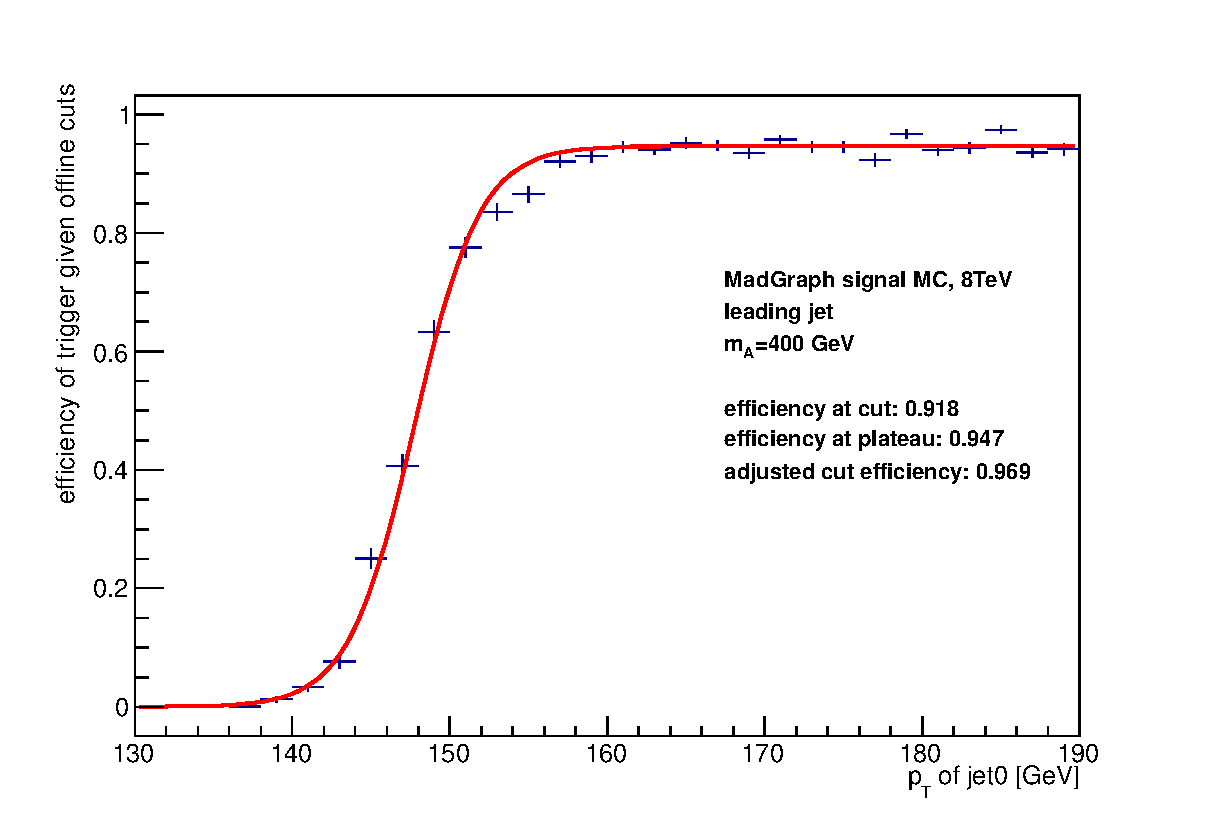
\includegraphics[width=\textwidth]{Systematics/images/jet0_trigger_turn_on_bAbb_400_j35.eps}\end{subfigure}
  \begin{subfigure}[sub-leading jet, $m_{A}=400$ GeV]{0.4\textwidth}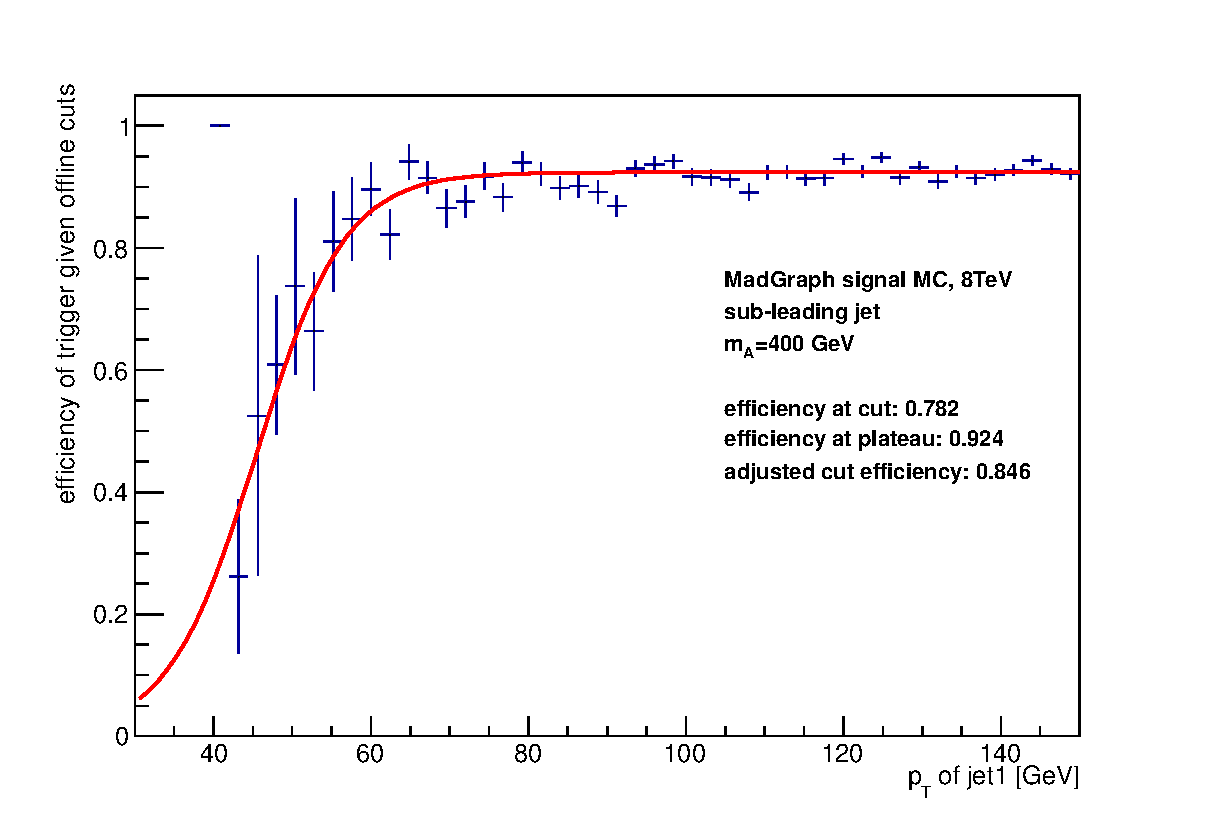
\includegraphics[width=\textwidth]{Systematics/images/jet1_trigger_turn_on_bAbb_400_j35.eps}\end{subfigure}
  \begin{subfigure}[leading jet, $m_{A}=450$ GeV]{0.4\textwidth}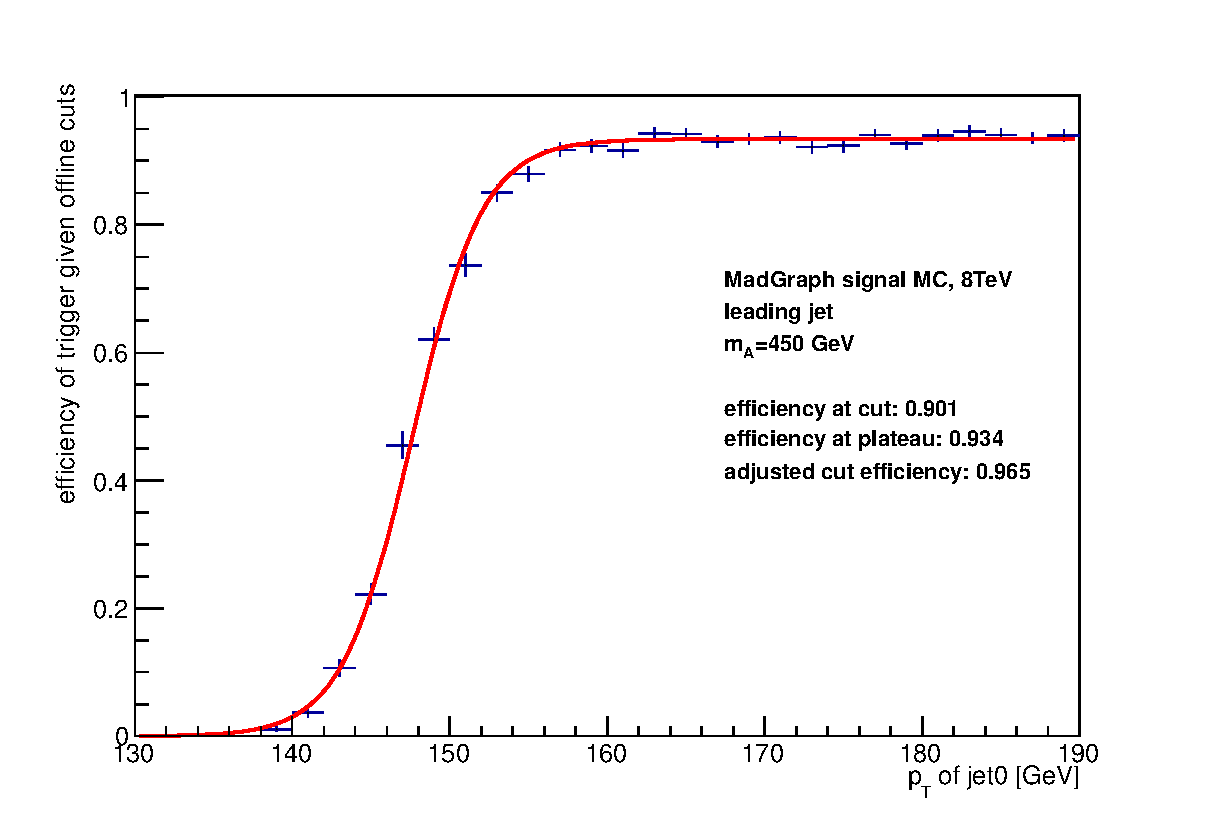
\includegraphics[width=\textwidth]{Systematics/images/jet0_trigger_turn_on_bAbb_450_j35.eps}\end{subfigure}
  \begin{subfigure}[sub-leading jet, $m_{A}=450$ GeV]{0.4\textwidth}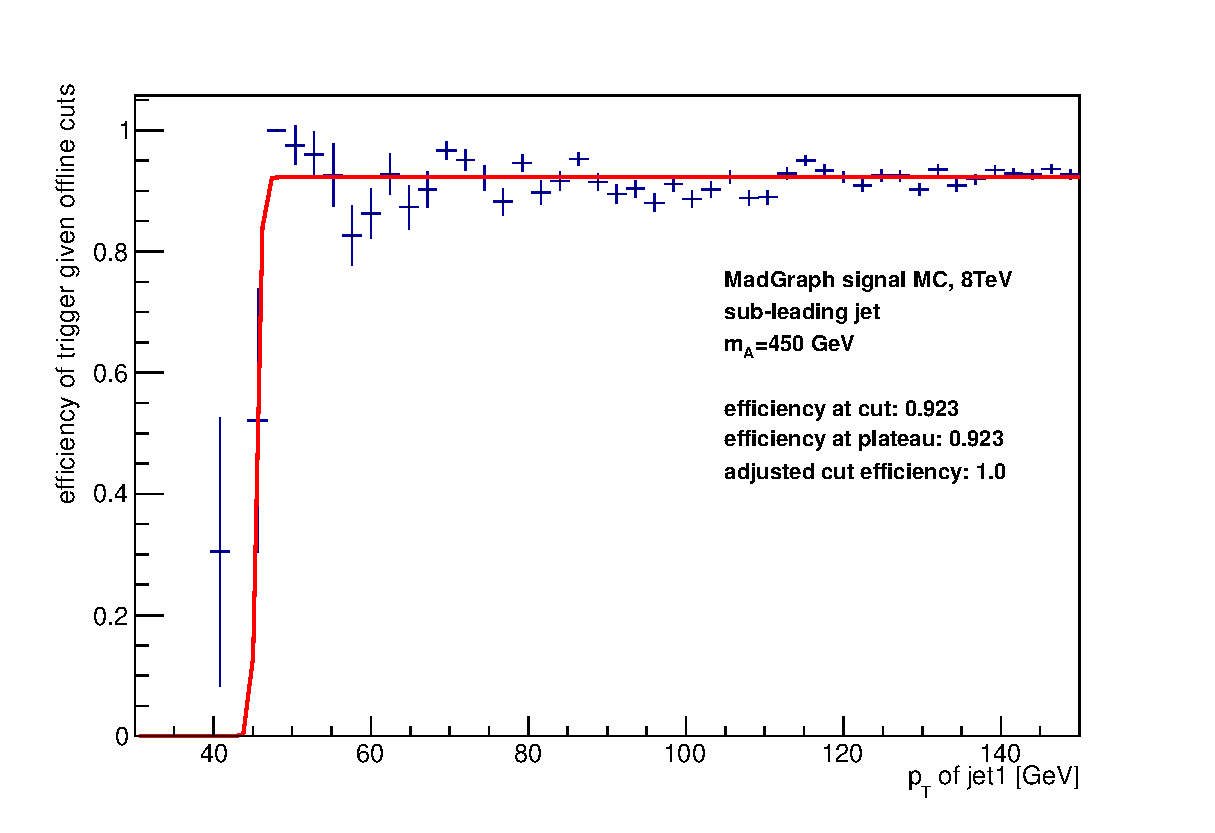
\includegraphics[width=\textwidth]{Systematics/images/jet1_trigger_turn_on_bAbb_450_j35.eps}\end{subfigure}
  \begin{subfigure}[leading jet, $m_{A}=500$ GeV]{0.4\textwidth}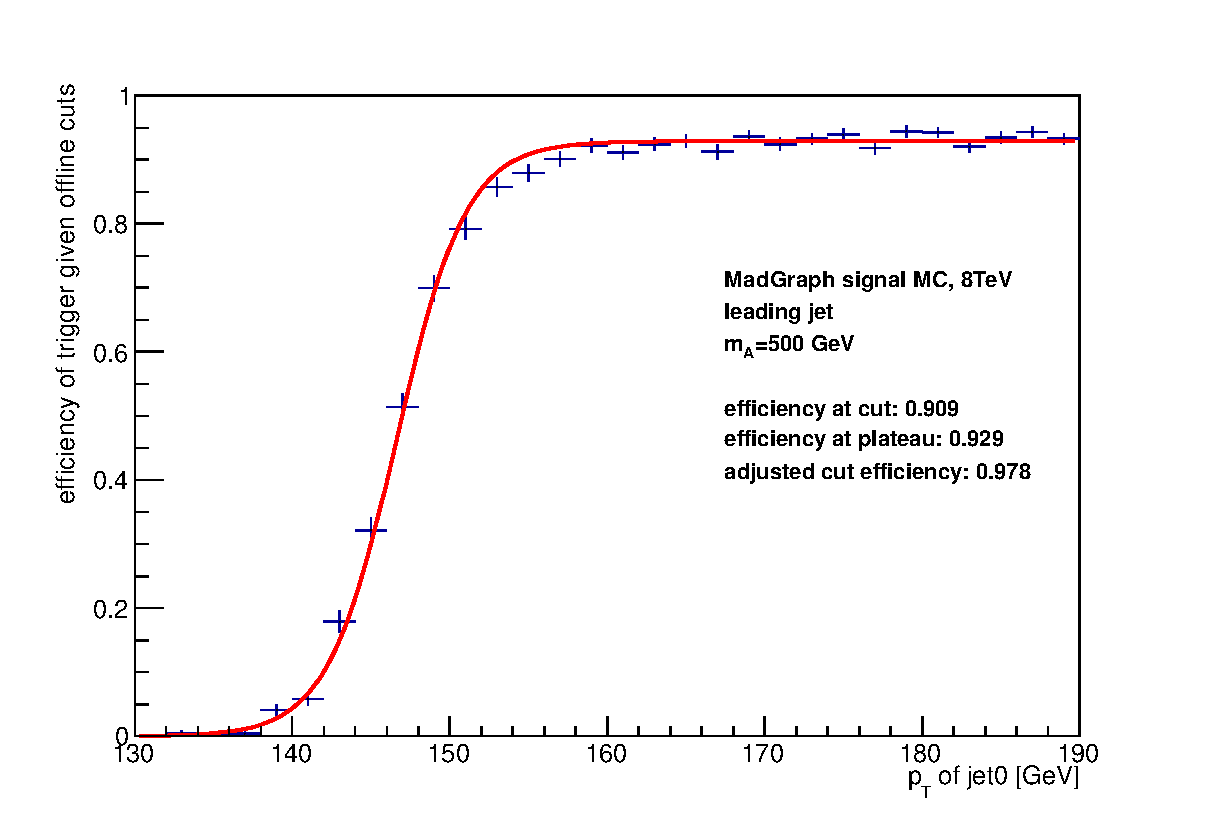
\includegraphics[width=\textwidth]{Systematics/images/jet0_trigger_turn_on_bAbb_500_j35.eps}\end{subfigure}
  \begin{subfigure}[sub-leading jet, $m_{A}=500$ GeV]{0.4\textwidth}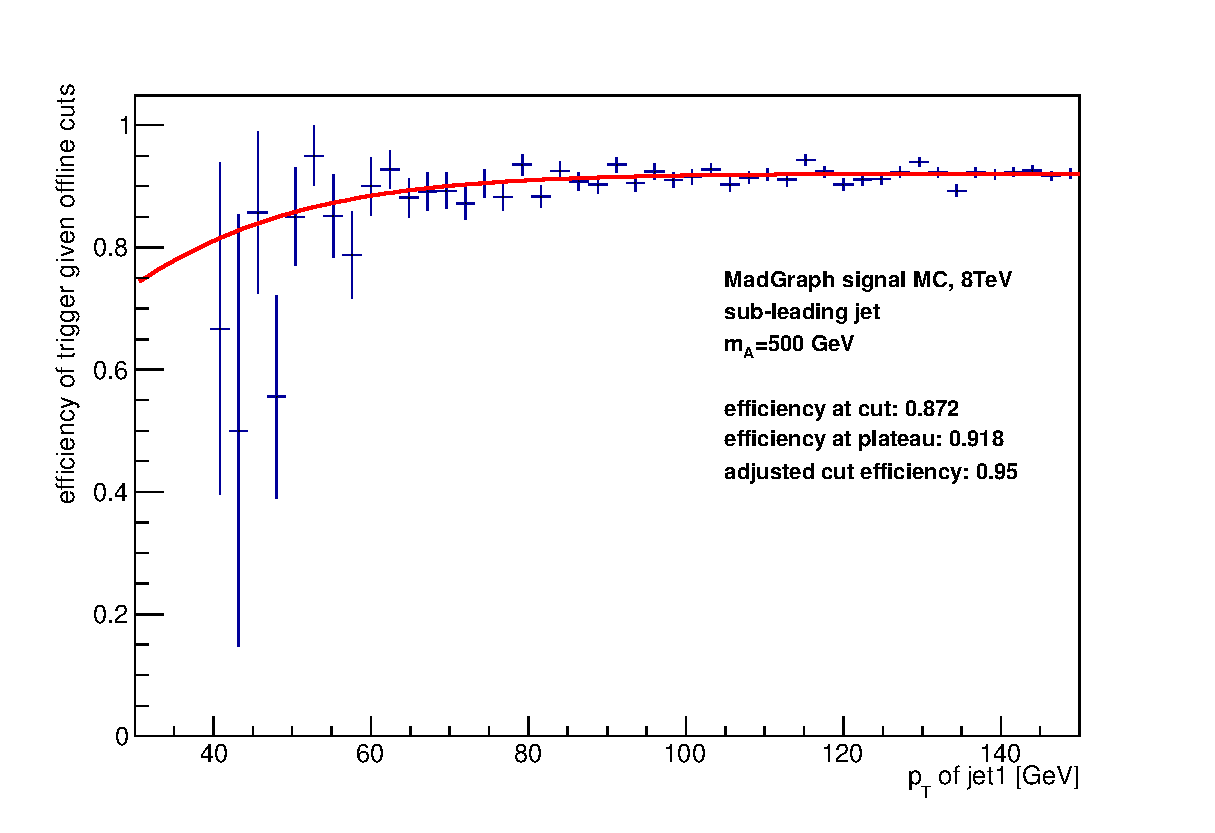
\includegraphics[width=\textwidth]{Systematics/images/jet1_trigger_turn_on_bAbb_500_j35.eps}\end{subfigure}
  \begin{subfigure}[leading jet, $m_{A}=550$ GeV]{0.4\textwidth}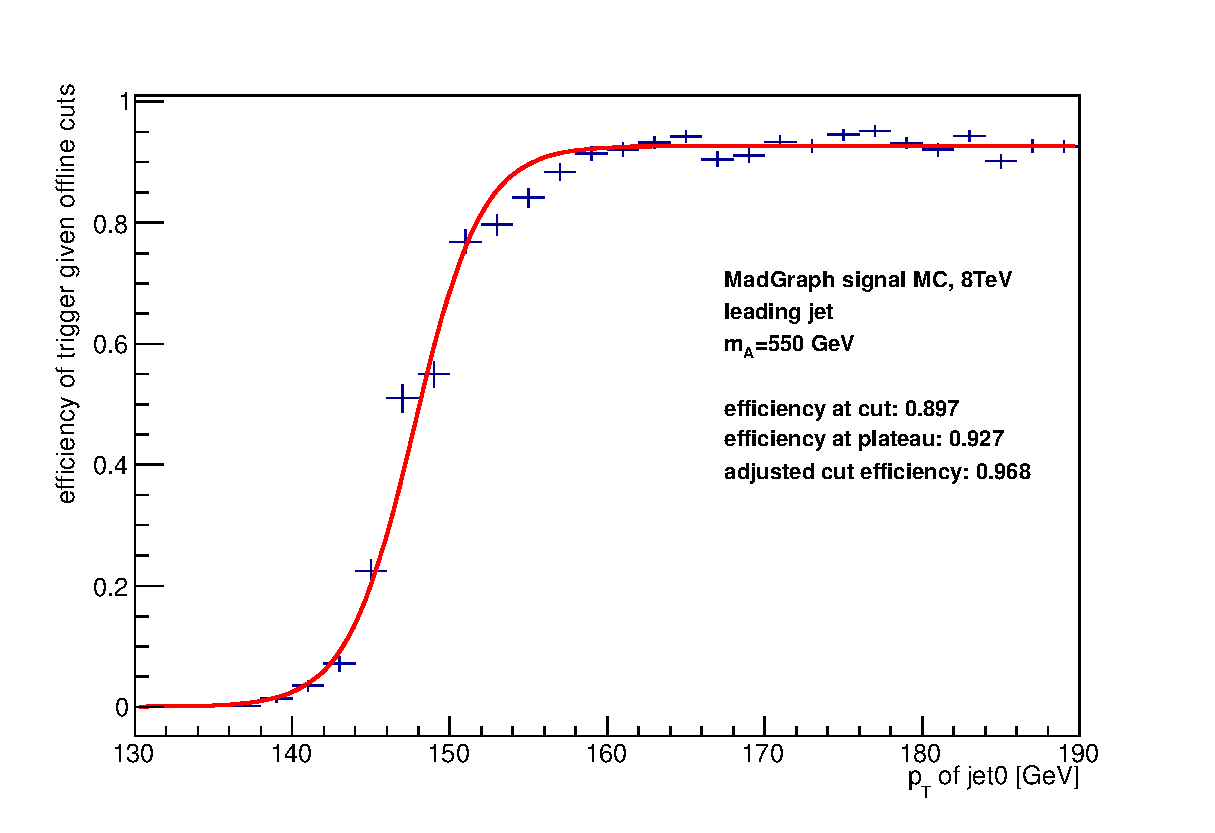
\includegraphics[width=\textwidth]{Systematics/images/jet0_trigger_turn_on_bAbb_550_j35.eps}\end{subfigure}
  \begin{subfigure}[sub-leading jet, $m_{A}=550$ GeV]{0.4\textwidth}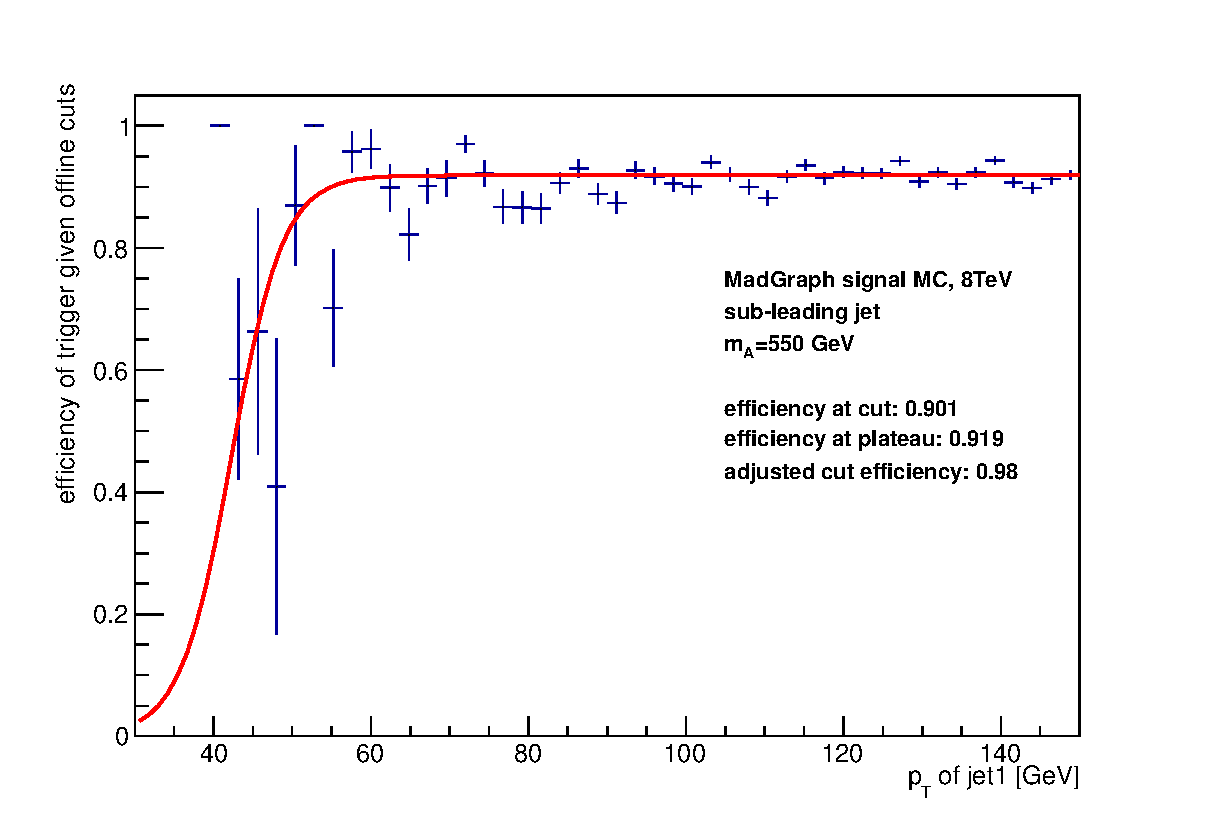
\includegraphics[width=\textwidth]{Systematics/images/jet1_trigger_turn_on_bAbb_550_j35.eps}\end{subfigure}
  \caption{The $p_T$ turn-on curves for the trigger for signal mass points 400-550 GeV.
  Although this search uses a multi-object trigger, in which several conditions 
  must simultaneously be true for a trigger acceptance, tight offline cuts can be used to isolate the effect 
  of a single jet's $p_T$ on the efficiency.  The curves are fit 
  with logistics, which are then used to extract the efficiency at the offline cut point, and to 
  adjust for any residual effects of other trigger objects that affect the efficiency. \label{fig:trigger_turn_on_1}}
    \end{center}
\end{figure}


\begin{figure}[phtb!]
  \begin{center}
  \begin{subfigure}[leading jet, $m_{A}=600$ GeV]{0.4\textwidth}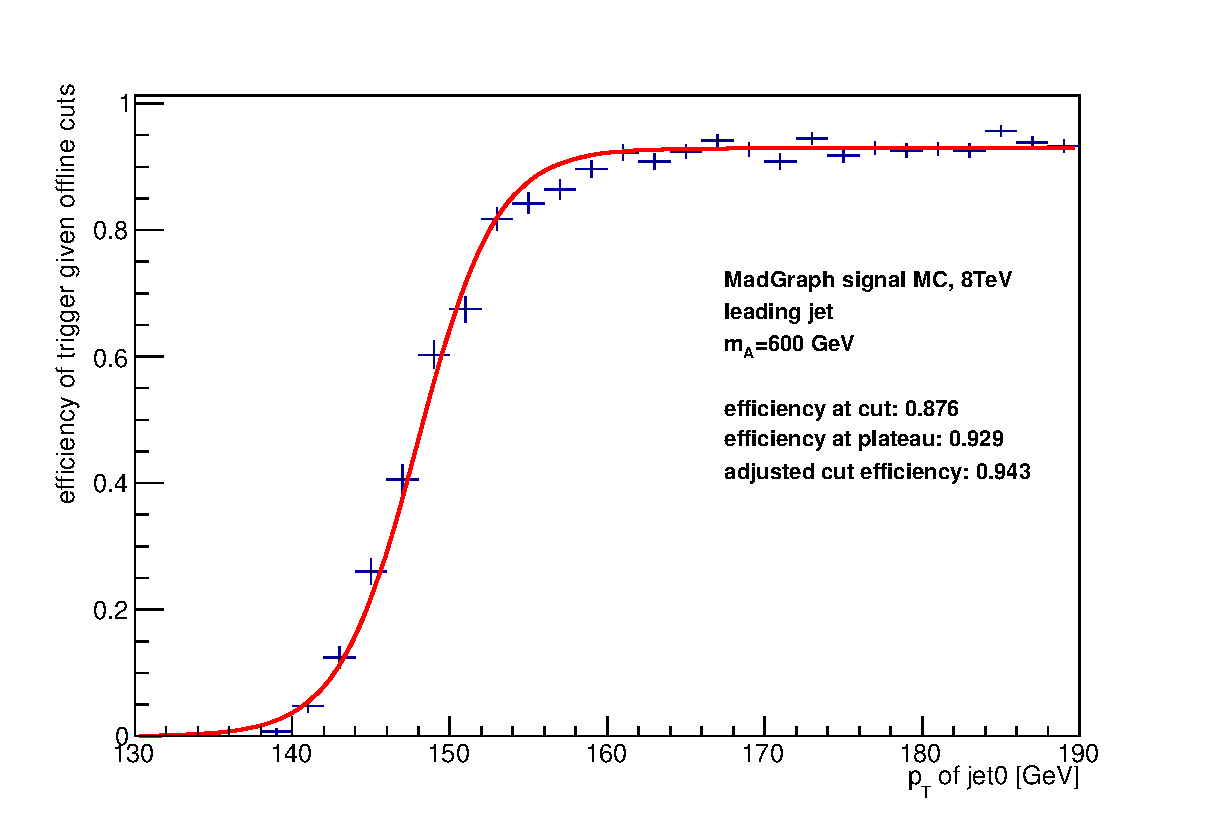
\includegraphics[width=\textwidth]{Systematics/images/jet0_trigger_turn_on_bAbb_600_j35.eps}\end{subfigure}
  \begin{subfigure}[sub-leading jet, $m_{A}=600$ GeV]{0.4\textwidth}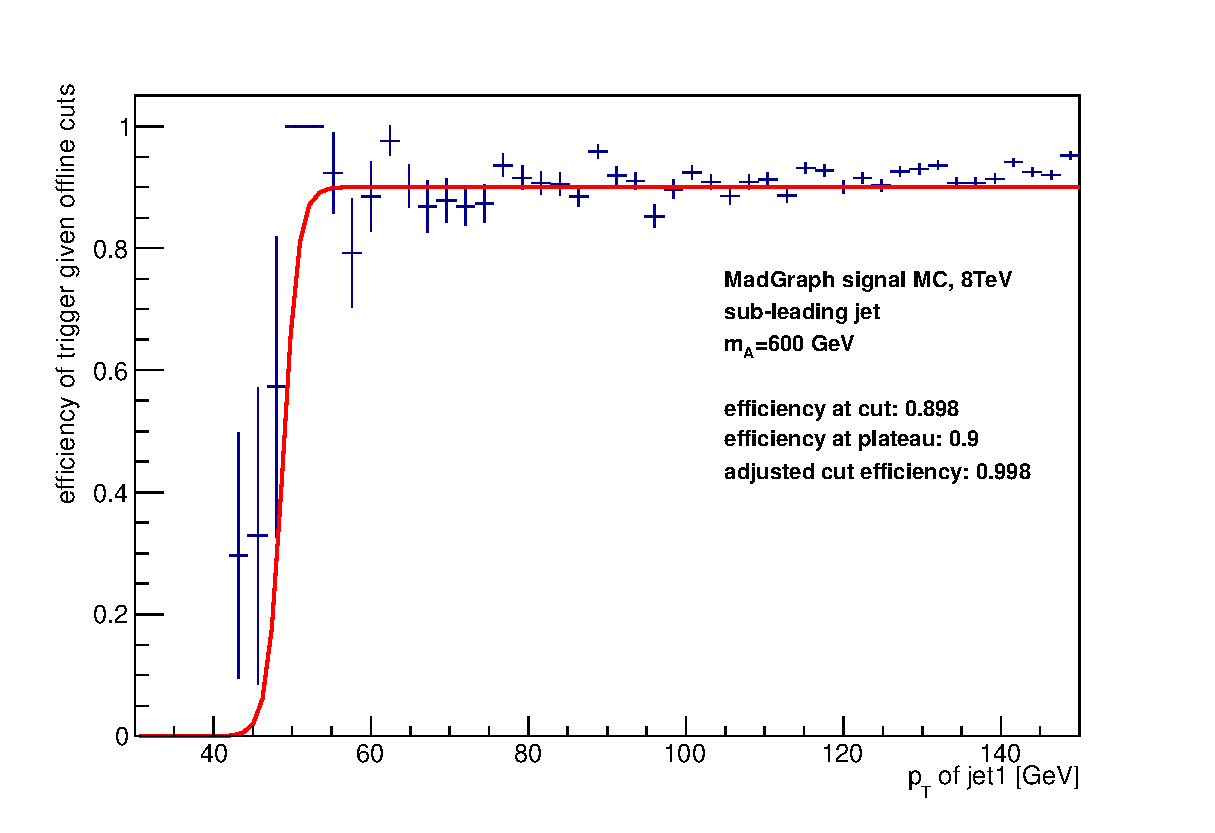
\includegraphics[width=\textwidth]{Systematics/images/jet1_trigger_turn_on_bAbb_600_j35.eps}\end{subfigure}
  \begin{subfigure}[leading jet, $m_{A}=650$ GeV]{0.4\textwidth}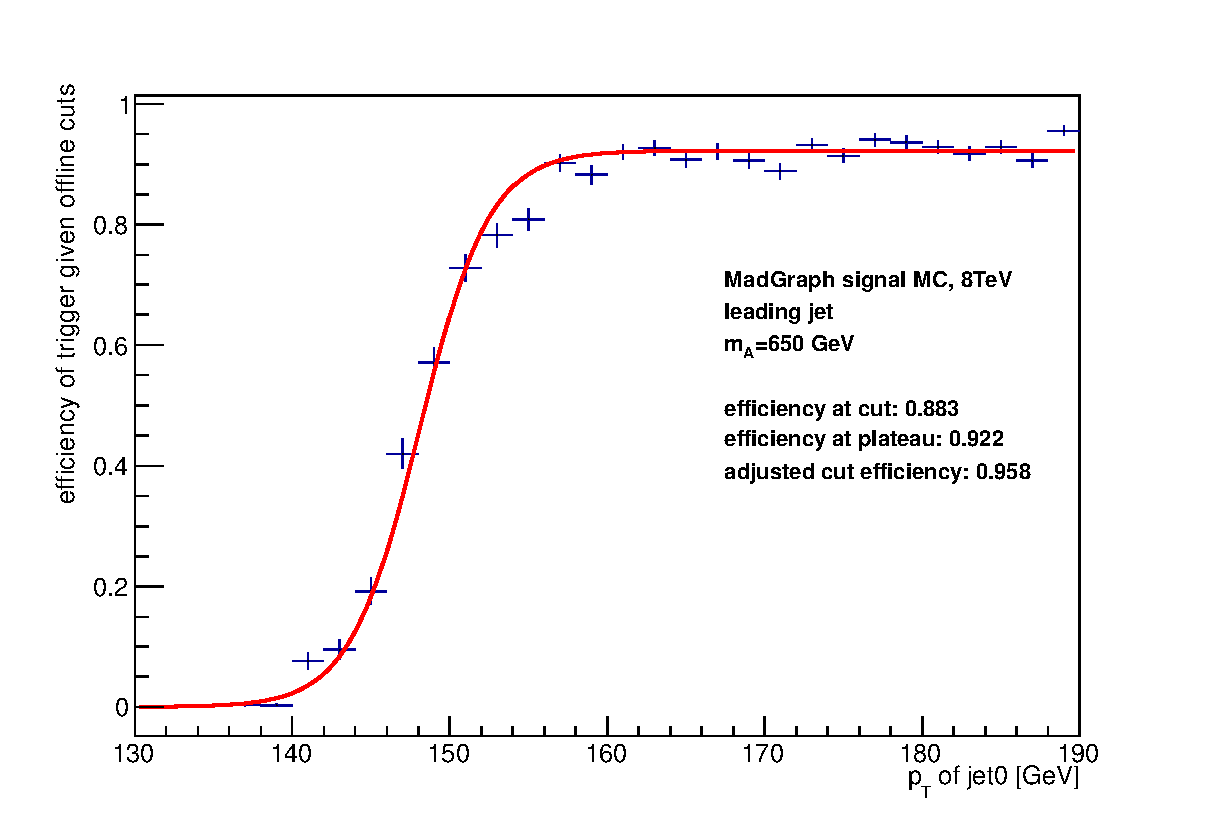
\includegraphics[width=\textwidth]{Systematics/images/jet0_trigger_turn_on_bAbb_650_j35.eps}\end{subfigure}
  \begin{subfigure}[sub-leading jet, $m_{A}=650$ GeV]{0.4\textwidth}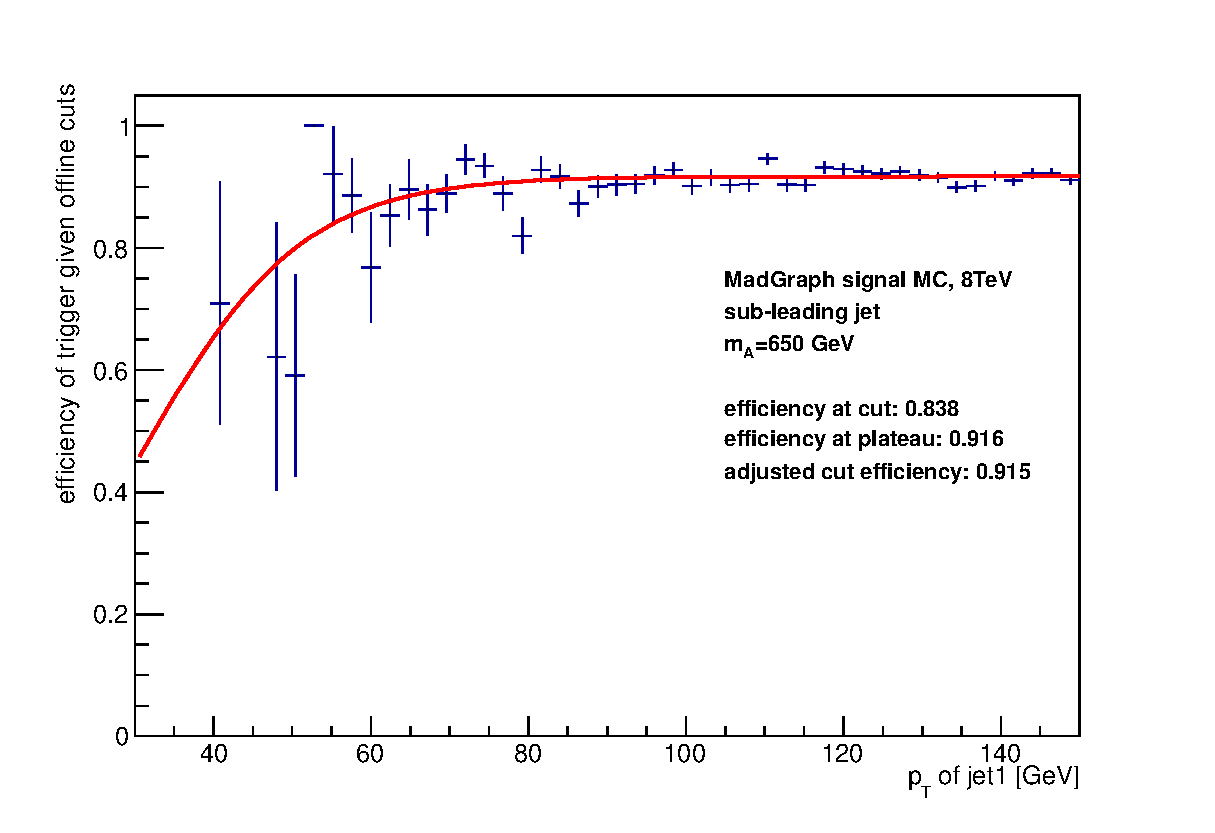
\includegraphics[width=\textwidth]{Systematics/images/jet1_trigger_turn_on_bAbb_650_j35.eps}\end{subfigure}
  \begin{subfigure}[leading jet, $m_{A}=700$ GeV]{0.4\textwidth}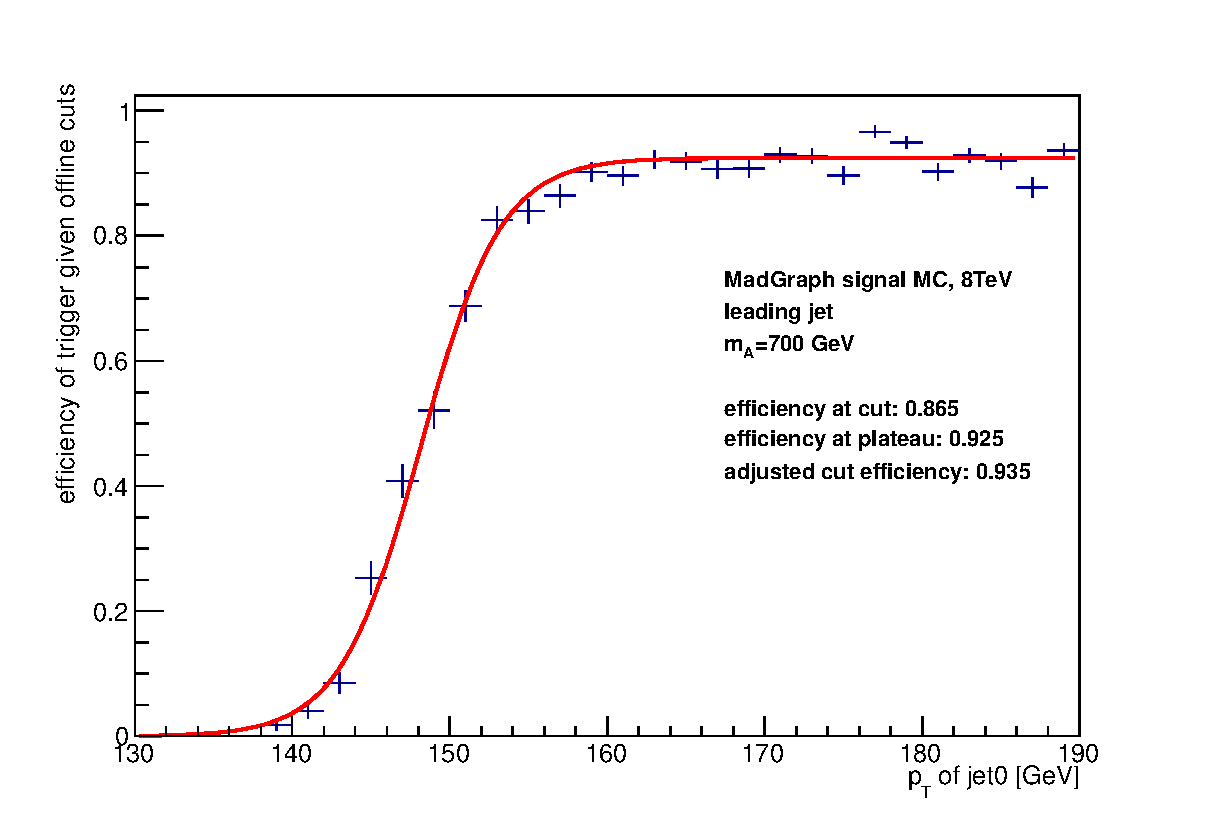
\includegraphics[width=\textwidth]{Systematics/images/jet0_trigger_turn_on_bAbb_700_j35.eps}\end{subfigure}
  \begin{subfigure}[sub-leading jet, $m_{A}=700$ GeV]{0.4\textwidth}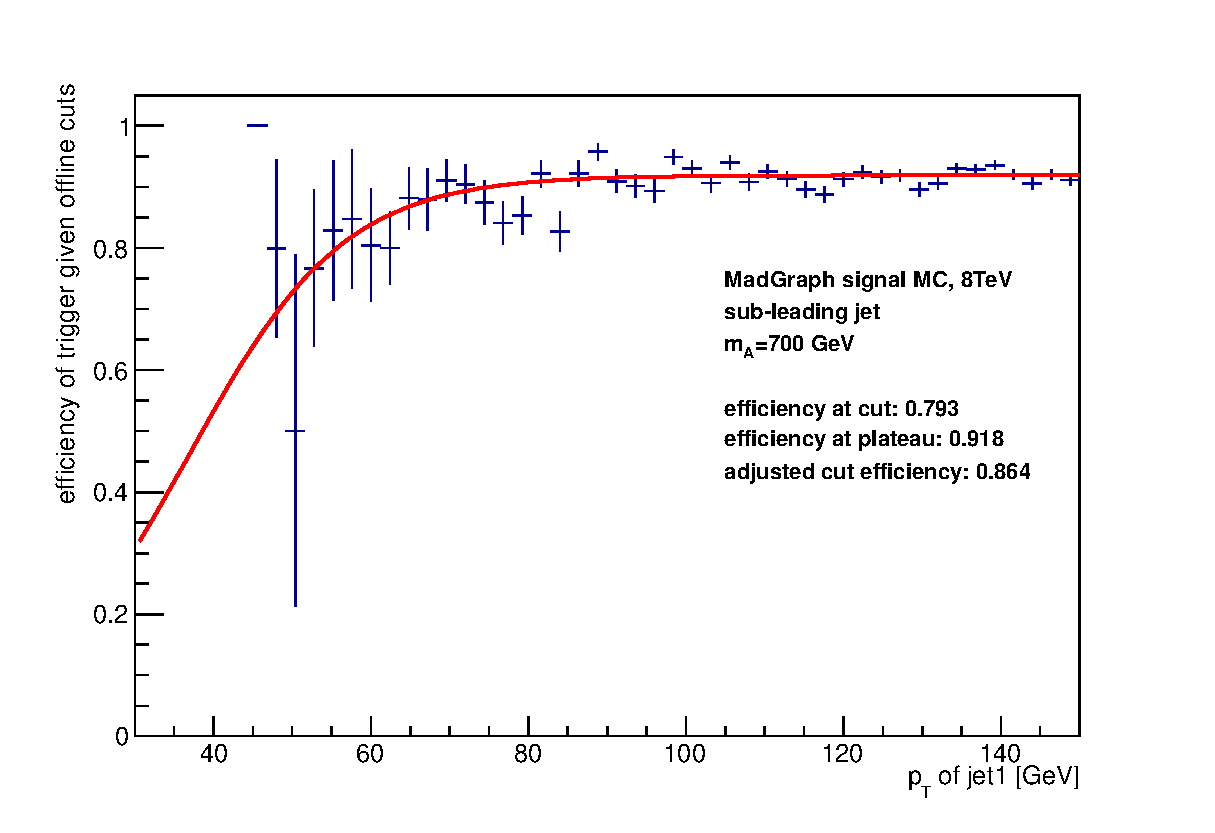
\includegraphics[width=\textwidth]{Systematics/images/jet1_trigger_turn_on_bAbb_700_j35.eps}\end{subfigure}
  \begin{subfigure}[leading jet, $m_{A}=800$ GeV]{0.4\textwidth}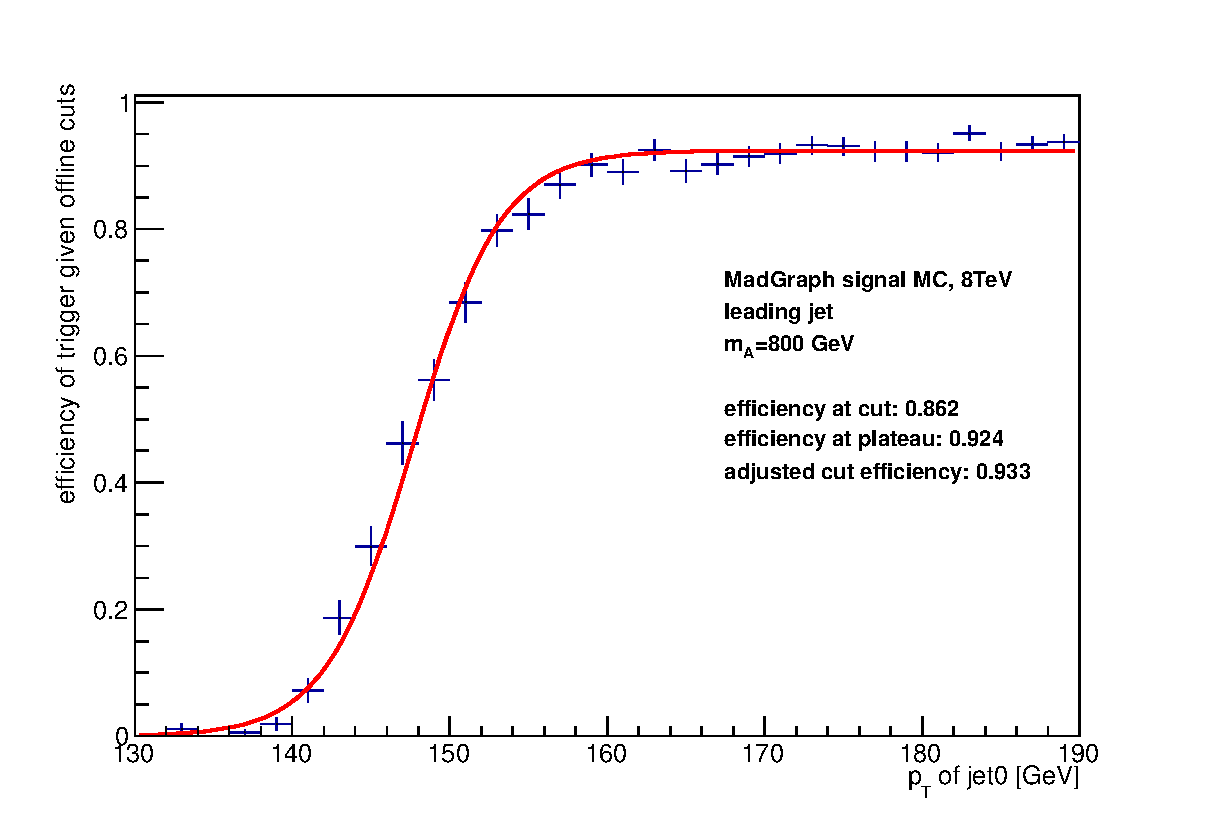
\includegraphics[width=\textwidth]{Systematics/images/jet0_trigger_turn_on_bAbb_800_j35.eps}\end{subfigure}
  \begin{subfigure}[sub-leading jet, $m_{A}=800$ GeV]{0.4\textwidth}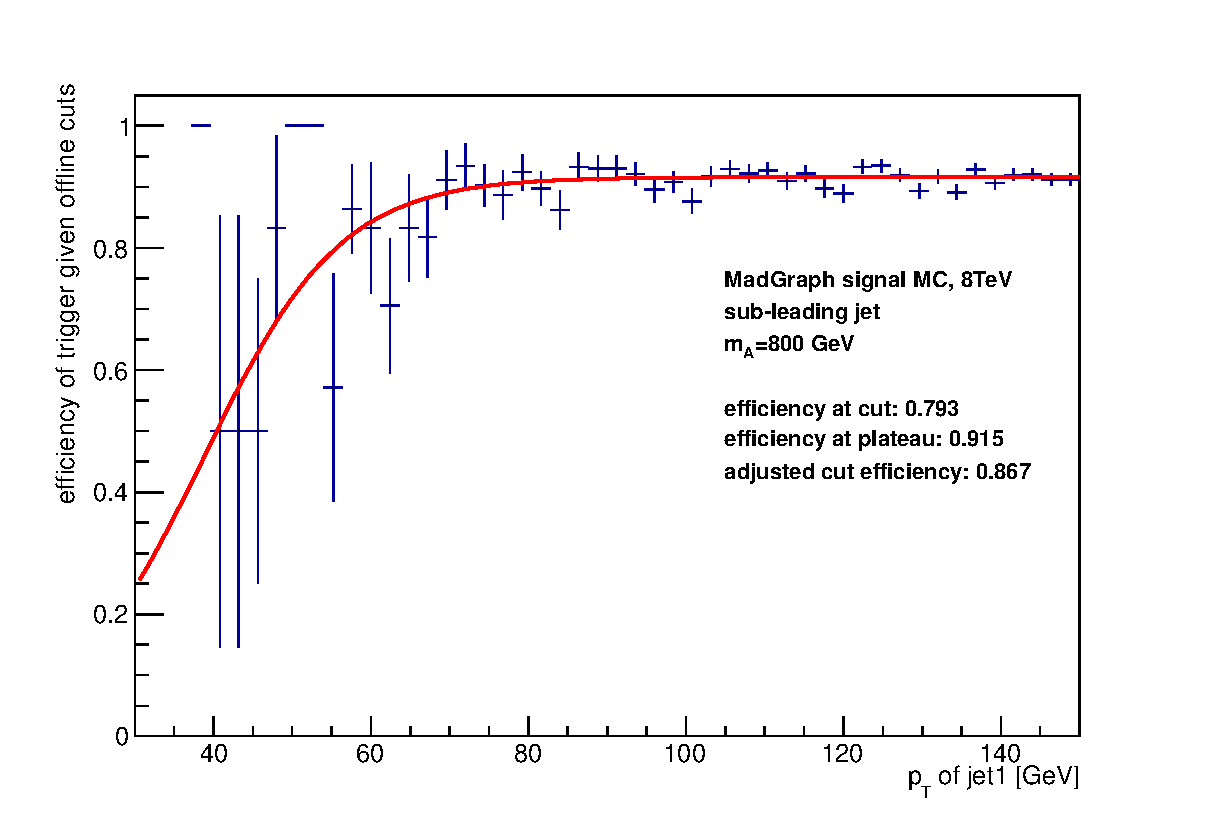
\includegraphics[width=\textwidth]{Systematics/images/jet1_trigger_turn_on_bAbb_800_j35.eps}\end{subfigure}
  \caption{The $p_T$ turn-on curves for the trigger for signal mass points 600-800 GeV.
  Although this search uses a multi-object trigger, in which several conditions 
  must simultaneously be true for a trigger acceptance, tight offline cuts can be used to isolate the effect 
  of a single jet's $p_T$ on the efficiency.  The curves are fit 
  with logistics, which are then used to extract the efficiency at the offline cut point, and to 
  adjust for any residual effects of other trigger objects that affect the efficiency. \label{fig:trigger_turn_on_1}}
    \end{center}
\end{figure}



\section{Jet Energy Scale and Resolution}
\label{sec:jes}
Hadronic particles fragment via QCD in the ATLAS detector, leaving deposits of 
energy in the calorimeters that must be clustered and reconstructed into jets.  The
observed jets then need some correction so that, on average, the reconstructed
jet energy corresponds to the energy of the associated stable particles.  The
calibration for this correction, called the jet energy scale (JES) and jet
energy resolution (JER), is calculated using MC simulations and then checked
in data.  The residual uncertainty on the JES and JER is then a systematic 
error on the analysis. 

The jet energy scale and its associated uncertainties are estimated using
in situ and test-beam-based measurements of isolated hadron response \cite{jes}.  The systematic
errors are integrated into the analysis via 14 independent variations, which are multiplicative factors applied to the jet
4-vectors and then the adjusted 4-vectors are run through the analysis framework.
The adjusted $m_{bb}$ distributions from the new 4-vectors are propagated through the fit as systematic
errors.  The effect of the jet energy scale varies depending on the signal mass
point, from about 3\% per variation at 400 GeV to $<$1\% at 800 GeV.

\textbf{add table here documenting the variations, their sources (i.e. what 
source of error they quantify) and effect per mass point}
%

\section{$b$-Tagging Scale Factors}
\label{sec:SF}
Although every effort is made to accurately simulate the production rates and
kinematic properties of $b$-quarks, as well as the performance of the ATLAS
detector, it is difficult to imagine that Monte Carlo simulation perfectly represents
the $b$-tagging efficiencies that might be found in data.  At the same time, it
is challenging to derive pure data-driven samples of $b$, $c$ and light jets to which
the b-tagging can then be applied, and used to derive the efficiencies:

    \begin{equation}
        eff_{b,c,light}=\frac{number\ of\ truth\ b,\ c,\ light}{number\ of\ tagged\ b,\ c,\ light}
    \end{equation}

Scale factors are computed by the flavor tagging performance group to quantify the
difference between the data and MC efficiencies.

    \begin{equation}
        eff_{data}=eff_{MC}\times SF_{data}
    \end{equation}


The scale factors are applied as events weights to the MC weight, where the value
of the scale factor depends on the $p_T$, $\eta$, $b$-tagging working point, 
 and truth flavor of the jet under
examination.  In practice, this means that the scale factors are binned in $p_T$
and $\eta$, with the $p_T$ bin edges at (), and the $\eta$ bin edges at ().
When there are multiple jets being examined for $b$-tags in a single
event, the net event weight is a product of all the relevant scale factors.
In this analysis, since only the first 5 jets are relevant for determining 
whether an event passes the analysis cuts or which $b$-tag category ($bbb$, 
$bbloose$, or $bbanti$), no scale factors are applied for jets that are 6th
or lower in the $p_T$ hierarchy of an event.

The scale factors are calculated by comparing the $b$-tagging efficiency computed 
in MC to the efficiency measured in carefully curated data samples, where the truth
flavor contents of the data are relatively well-known \cite{b-tagging}.  For the $b$-jet
scale factors, a sample of $t\bar{t}$ events is used for the data component; for 
$c$-jets, the calibration is done with $D^*$ events.

The scale factors are used to correct the MC $b$-tagging performance back to the $b$-tagging
behavior seen in data, but the calibration process can introduce systematic uncertainties
that have to be quantified and propagated through to the final result.  The $b$-tagging
systematics are computed and applied using a method called the eigenvector method.
The eigenvector method is used to derive a set of independent variations of the data-MC scale
factors, in such a way to take the full covariance matrix of the calibration measurements
into account, including correlations among working points and different jet $p_{T}$ regions.
For further explanation of the eigenvector method please see section 2.3 of \cite{VHBTagging}. 


The presence of $b$-tagging in the trigger means the sample of data collected for this 
analysis is already enriched in jets that look more $b$-like, so the scale factors
are different based on how a jet is tagged (online, offline, or both). 
The calibration procedure takes this into account, by using the following algorithm
to compute the scale factors:
\begin{enumerate}
    \item Separate MC jets by whether they are $b$-tagged offline
    \item If they are $b$-tagged offline, separate by whether they are 
        also $b$-tagged online
    \item Repeat these steps, but with data
    \item In each possible permutation (online+offline, online-only, offline-only)
        compute MC/data scale factors for the jets in that category 
\end{enumerate}


\textbf{add in a picture of the b-tag weight distributions}



%Gto be aroundP Soon we can reference the cont. tagging conf note (for now ATLAS-COM-CONF-2014-003).





%\begin{figure}[hbt]
%  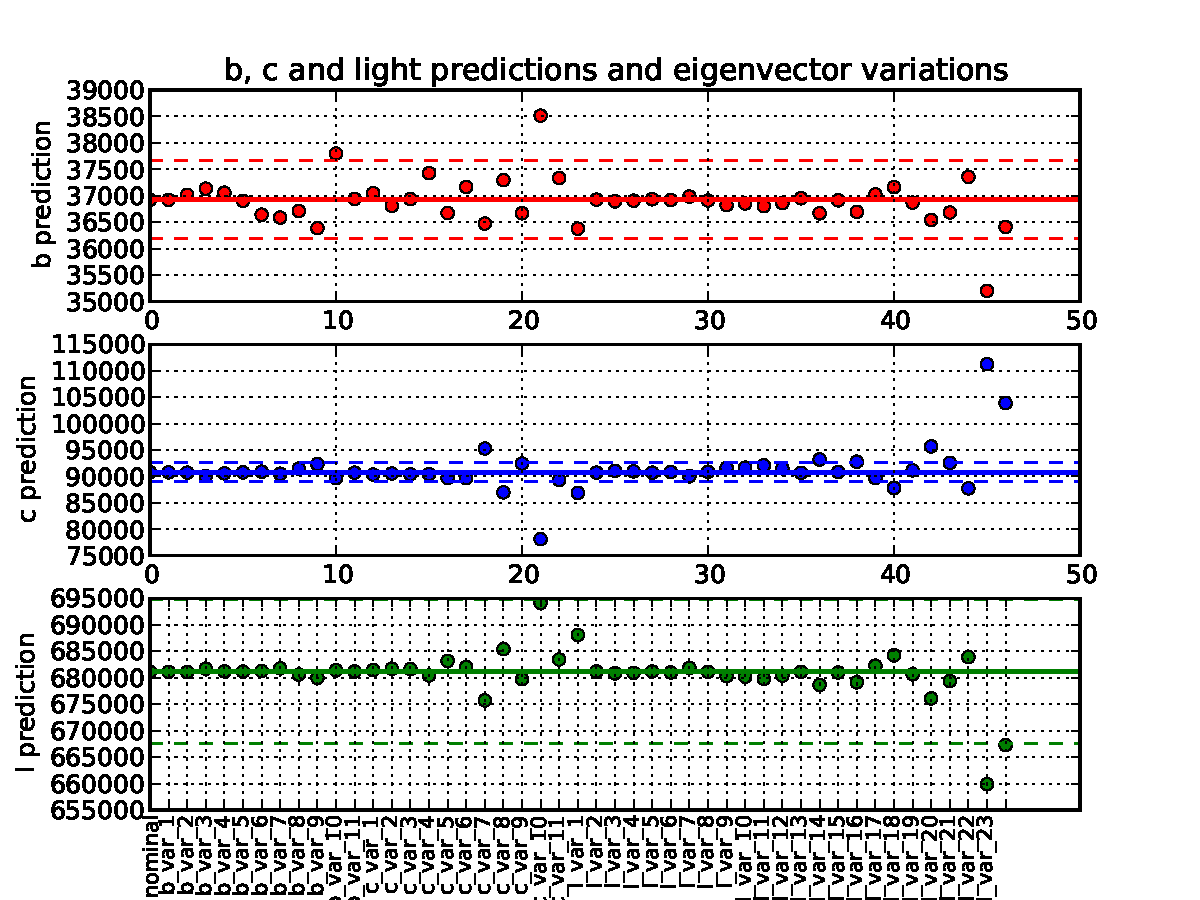
\includegraphics[width=0.98\linewidth]{Systematics/eigenvector_variations.pdf}
%  \caption{The changes in flavor predictions in data due to eigenvector variations.  Th
%    colored line in each subplot shows the nominal prediction given by the matrix method;
%    each point is the prediction generated when a different eigenvector variation is applied.
%    The variations are labeled on the x axis.  The colored dotted lines show the +\- 2\%
%    envelope for the nominal prediction.}
%  \label{fig:eigenvector_variations}
%\end{figure}





%\subsection{Systematic Errors on Data-Driven Background Estimates}
%Validating the matrix method predictions of the $m_{bb}$ shap is a bit more subtle. 
%Since we use the matrix method to help validate our assumption that mbb of the leading 2 jets is independent of the truth
% flavor of the third jet, we need to demonstrate that the matrix method reweighting does not distort the
% mbb shape. We test this by generating toy MC distributions where our assumption is incorrect (by design,
% we make the mbb distribution dependent on the truth flavor of the 3rd jet) and then run those toy events
% through the matrix method to check if the different distributions are projected out correctly.
% Using the $m_{bb}$ distribution in data as a template, we generate three $m_{bb}$ distributions that have different
% shapes (the $m_{bb}$ values are scaled down by 7\% for light jets, left unchanged for charm jets, and scaled
% up by 15\% for bottom jets), and draw an $m_{bb}$ value at random from one of those distributions depending
% on the truth flavor. These different $m_{bb}$ distributions are not meant to model the data in any physically
% relevant way, but rather to guarantee that if there are systematic differences in $m_{bb}$ that are correlated
% with the flavor of the third jet, the matrix method will get the $m_{bb}$ shape correct.
% The results of this study can be seen in Figure~\ref{fig:mbb_compare_truth_mm_toy}; it is clear that the 
%shape differences in the original distributions propagate through to the matrix method predictions.



%\begin{figure}
%    \centering
%    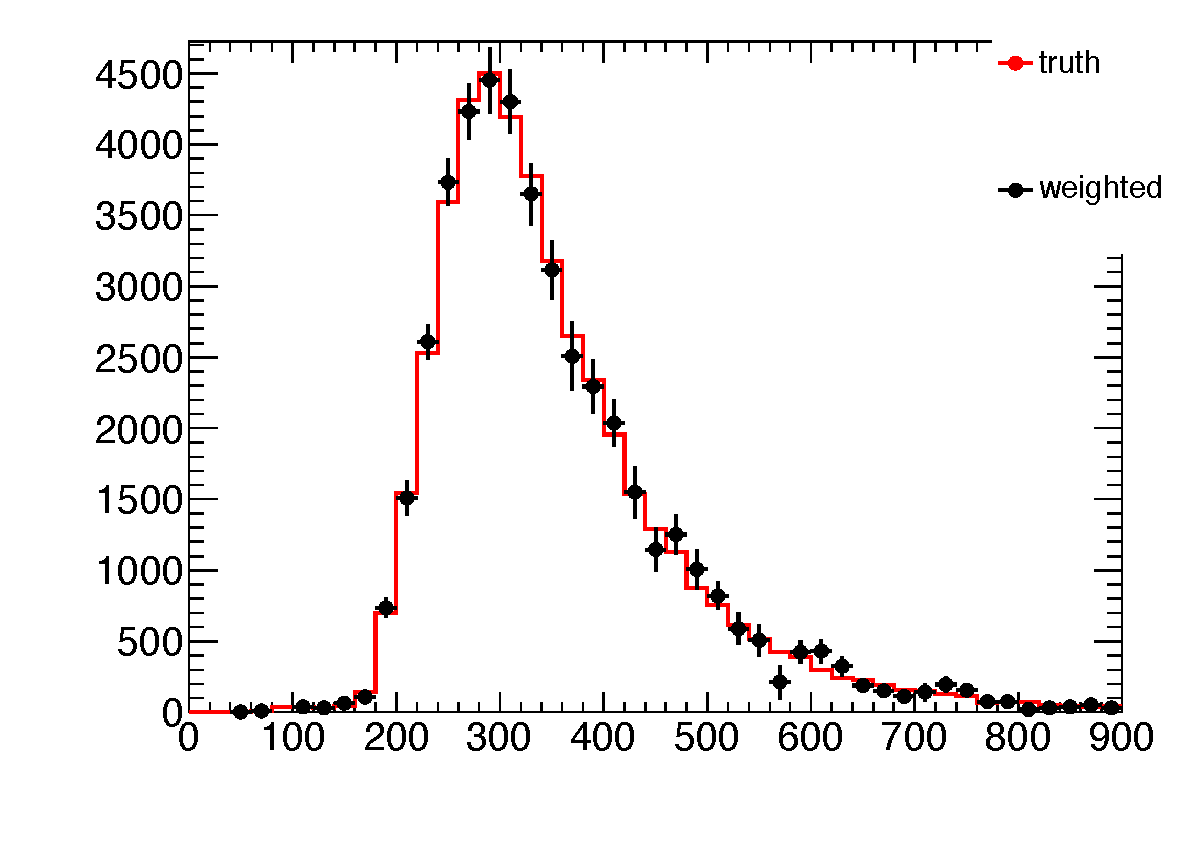
\includegraphics[width=0.3\linewidth]{Systematics/mm_shape_check_b.pdf}
%    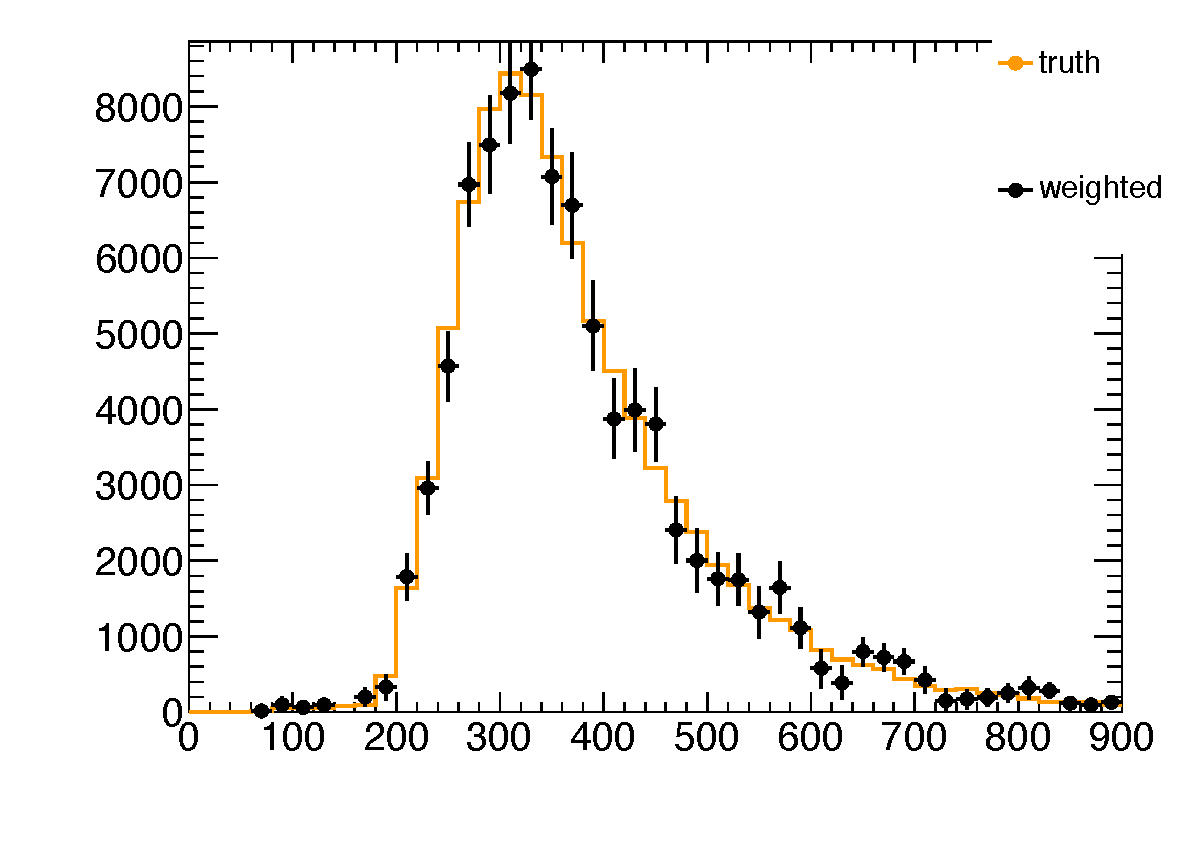
\includegraphics[width=0.3\linewidth]{Systematics/mm_shape_check_c.pdf}
%    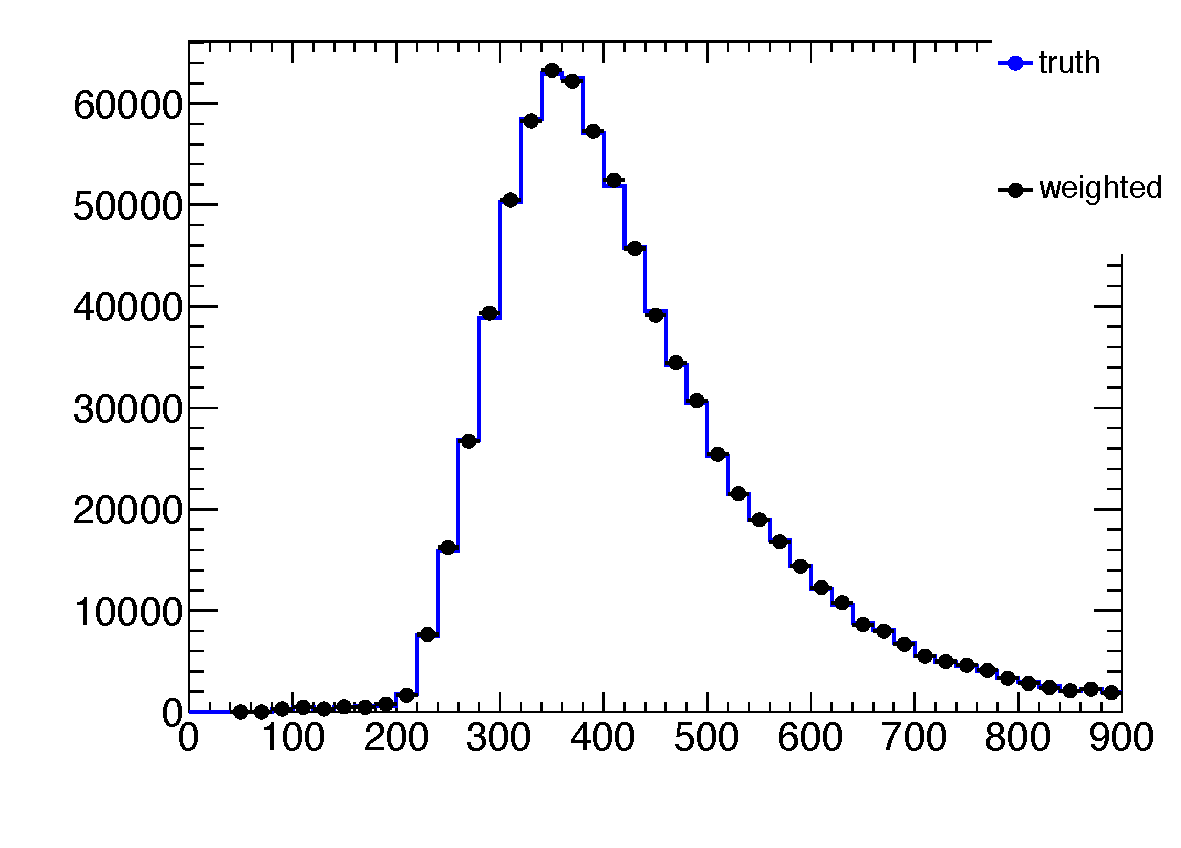
\includegraphics[width=0.3\linewidth]{Systematics/mm_shape_check_light.pdf}
%    \caption{A comparison of the toy $m_{bb}$ distributions for the different flavors of the
%        third jet, as shown in Figure~\ref{fig:mbb_compare_truth_spectra}, with the matrix
%        method predictions overlaid.  }
%    \label{fig:mbb_compare_truth_mm_toy}
%\end{figure}

